\chapter{Prototype implementation}\label{chap:impl}
This chapter describes how the essential parts of the designs outlined in previous chapters were fulfilled in practice by implementing a proof-of-concept interpreter and development environment.

\section{Programming discipline}
The prototype was implemented largely in the spirit of exploratory programming:
``the kind where you decide what to write by writing it.''\cite{arc}.

This approach in combination with a dynamic and flexible language like
JavaScript enables one to quickly transform ideas to working prototypes and
shape them as one goes along. But the usefulness of this method is limited, as
it may quickly produce fairly low-quality code, as it is not focused on future
maintainability.

Most of the features of the prototype system are implemented as a proof-of-concept, were the main focus is making them work. Performance and other considerations are of low priority. Some features are more refined than others in order to fulfil the major goals of this thesis, one of which was to implement a working non-trivial application in the language.

\section{The language}
The language's parser and interpreter are implemented in JavaScript. The parser conforms to the grammar specification described in Section \ref{sub:basic_syntax} with all of its extensions defined in Chapter \ref{chap:lang}. The parser emits events while processing every language construct. These events carry individual syntax tree nodes with information about the current position in the source string. The events are then captured by the environment to attach additional information to \acrshort{est} nodes, such as references to elements of the visual representation (\acrshort{dom} nodes), and objects that represent text fragments.

The prototype implementation of the language contains all the features described in Chapter \ref{chap:lang}, with the following exceptions:
\begin{itemize}
    \item Macros are not implemented.\footnote{In fact, they partially \textit{are} implemented, but are not usable. For example, there is a \texttt{macro} primitive available, which produces macro values. But it should not be used, as these macro values are not treated specially by the interpreter, so using them will not have the desired effect.}
    \item There are two primitives, which produce function values: \texttt{of} and \texttt{of-p}. The second has the same meaning as \texttt{of} described in Chapter \ref{chap:lang}. The first has the same meaning, except that it does not use pattern matching when binding names to arguments. This primitive requires that all the names must be words.
    \item Destructuring is implemented only for definitions (it works in \texttt{bind}) and not for assignments (it does not work in \texttt{mutate}). Pattern matching could easily be extended to mutation, although I have found it sufficient to be usable only in definitions and ended up not implementing it for assignments in the prototype.
    \item Comments are treated and attached to \acrshort{est} nodes as streams of characters. Nesting and balancing of brackets is taken into account in multi-line comments, but their tree-like structure is not preserved.
    \item Strings are not treated specially by the parser. They are stored and manipulated as syntax tree nodes, not as streams of characters. This means that the optimization described in Section \ref{sub:str} is not applied. The performance penalty is acceptable in the prototype implementation. 
    \item The escape character \texttt{\textbackslash} has no special meaning. To substitute a special character in a string, the following built-in values are defined:
    \begin{lstlisting}
    (left-bracket) -- escapes "["
    (right-bracket) -- escapes "]"
    (left-brace) -- escapes "{"
    (right-brace) -- escapes "}"
    (pipe) -- escapes "|"
    (bang) -- escapes "!"
    \end{lstlisting}
    
    So \texttt{'[(left-bracket)hello(right-bracket)]} would evaluate to: \texttt{"[hello]"}.
\end{itemize}

The interpreter is implemented naively. Its main part is the recursive \texttt{evaluate} function. The function accepts an \texttt{expression} and an \texttt{environment}. The expression can be a number literal, an identifier or an invocation. Each of these types is evaluated differently:
\begin{itemize}
\item If it is a number literal, it evaluates to its corresponding numerical value.

\item If it is an identifier (a name), it is looked up in the environment and the corresponding value is returned. If it is not found in the environment, an error is thrown.

\item If the expression is an invocation then it is evaluated according to its operator:
\begin{itemize}
\item If the operator is a string operator \texttt{'} or \texttt{html'}, then first any variable substitutions are performed and then the corresponding string value is returned.
\item If the operator is a primitive, then the expression's arguments are not evaluated and passed to this primitive, which may or may not evaluate them. The result of the primitive's application is returned.
\item If the operator is an expression, then it is evaluated. Then its arguments are evaluated. If any of those arguments is a substitution expression (i.e. it is wrapped in curly braces \texttt{\{\}}) then it is expanded before proceeding. When all of the arguments are evaluated, the operator is applied to them and the result of this application is returned.
\end{itemize}
\end{itemize}   

%Lisp's syntax is as minimal as it gets\cite{syntaxation}, which makes 
%There are many approaches to implementing interpreters for LISP in JavaScript\cite{js_lisps}, but the general principles are the same.

\section{The environment}
The development environment's prototype implementation provides only the few critical features that are necessary to demonstrate how complete integration and interchangeability of the text and visual representations of the language can be achieved.

The prototype of the environment has elements of a web application in its implementation. However, it is prepared only to work offline, on the user's machine.

The system is implemented with minimal dependencies, so it can be easily
installed and so that a greater level of integration can be achieved by having more control over every part of the system.

The only required dependencies for the basic functionalities of the prototype to
work is a web browser and the CodeMirror library. An additional dependency is the Node.js environment -- for running the stub of the project manager.

\begin{figure}[h!]
\centering 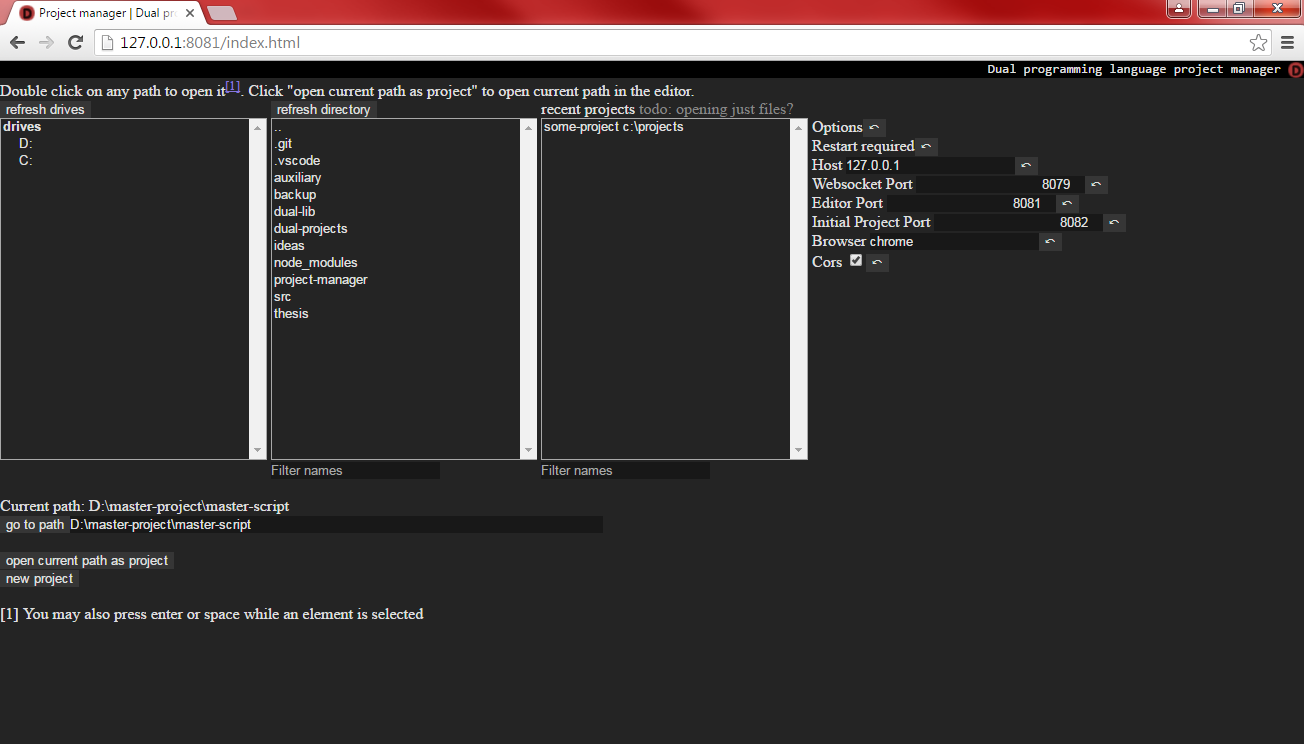
\includegraphics[width=0.9\textwidth]{project_manager}
\caption{Dual's project manager}
\label{fig:project_manager}
\end{figure}

\begin{figure}[h!]
\centering 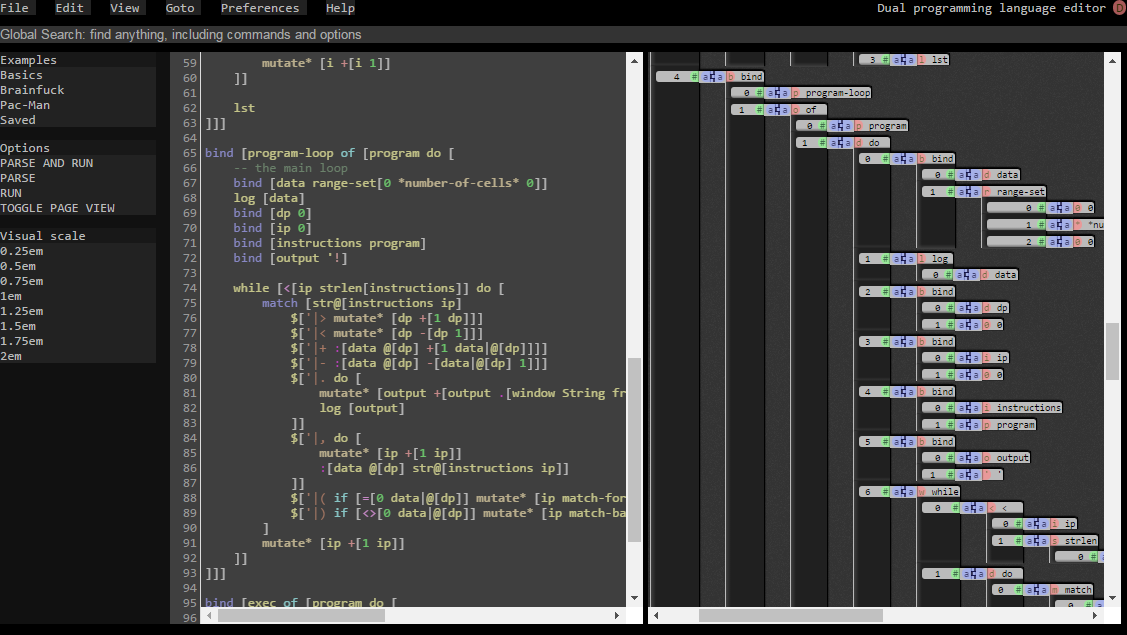
\includegraphics[width=0.9\textwidth]{editor}
\caption{Dual's editor}
\label{fig:editor}
\end{figure}

\subsection{General architecture}
The development environment's web-application-like architecture is reflected in its three main components:
\begin{itemize}
    \item The server part, implemented in JavaScript on top of Node.js. This
      part's function is mainly to enable access to the user's file system, so that any local folder can be opened as a project. Modern web browsers restrict access to the local file system, as dictated by their security policy. The server part also handles persisting changes to files and configuration.
    \item The project manager part, which communicates directly with the server
      part. The connection is maintained over a WebSocket\cite{mdn_websockets}. This part provides access to user's file system via a custom folder selection interface. Basic configuration of server communication, such as changing the address and ports is also possible. Once a project is selected, the user may open it in the editor part. Figure \ref{fig:project_manager} demonstrates the interface of the project manager.
    \item The editor part, which is the main component and can function as a
      stand-alone application. It can communicate with the server indirectly,
      through the \texttt{localStorage} mechanism\cite{mdn_localstorage}.
\end{itemize}

The project manager and the editor, which can be considered the front-end parts
of the system are designed to be \acrlong{spa}s\cite{spa_wikipedia}. The
project manager exchanges JSON messages with the server through a WebSocket. This is used for updating the view with dynamic data. In order to facilitate the manipulation of the HTML structure of the page, which is the main application's view, I implemented a very simple web application framework, which
binds the data from the server with the data on the client and the
\acrlong{dom}\cite[Chapter~13]{eloquentjs}.

Figure \ref{fig:editor} shows an overview of the editor prototype's window. The
basic layout is modeled after the aforementioned code editors. At the top of the
window is the menu bar, below it a mockup of a global search input (not implemented). The left panel contains basic controls for selecting examples,
invoking the parser and interpreter, toggling application view and adjusting the
scale of the visual representation.

The browser's JavaScript console is used as the standard output. There is no built-in console.

The following options are implemented in the prototype:
\begin{itemize}
    \item Available from the menu bar:
    \begin{itemize}
        \item File->Save, which saves the current content of the text editor to
          a file named \texttt{save.dual} in editor's root directory. This only
          works if the server-side part of the environment is running. Otherwise
          the source will be saved only to browser's internal storage.
        \item In the Edit menu: Undo, Redo, Cut, Copy, Paste and Select All
          options are supported. Note that by default web browsers restrict the
          access to the user's clipboard, so for Copy and Paste the standard key
          shortcuts should be used (Ctrl-C, Ctrl-V). All other conventional
          keyboard shortcuts are also supported, thanks to the CodeMirror
          library.
    \end{itemize}
    \item Available from the left panel:
    \begin{itemize}
        \item The options in the Examples submenu cause a corresponding source
          file to be loaded into the editor. This is for demonstration for the
          purposes of this thesis.
        \item The Options submenu allows the user to invoke the parser and the
          interpreter separately or in combination as well as toggling between
          the ``page'' (also known as ``application'') and visual editor
          views. The application view contains an embedded web page (iframe),
          which can be manipulated by a Dual application. This is used to
          display the game view in the Pac-Man clone example.
        \item The Visual scale submenu changes the size of the blocks in the
          visual editor. This demonstrates how manipulating one CSS property
          influences the rendering of the visual representation.
    \end{itemize}
\end{itemize}

Some options have descriptive captions available that appear when the mouse
cursor hovers over them.

\subsection{Text editor}
The text editor is built on top of the CodeMirror framework\cite{codemirror_site}. This provides all basic features of a text editor, such as automatic indentation, syntax highlighting (a custom syntax highlighting mode for Dual is defined), line numbering, block selection or parallel editing of multiple lines.

The text editor is integrated with the environment. The fragments of text corresponding to EST nodes in the text representation are tracked by CodeMirror's TextMarker objects. These facilitate tracking and propagating any changes to and from this representation, as well as highlighting of the currently focused expression.
      
If a position of the text cursor in or the contents of the source change, a fragment of text corresponding to the appropriate \acrshort{est} node is highlighted. Also the corresponding subtree in the visual editor is highlighted. It works also in the other direction -- when a node in the visual editor is selected, it is highlighted along with the corresponding text fragment.

This demonstrates the core functionality of the system: it is ``aware'' at all times of currently focused meaningful part of the code, corresponding to an \acrshort{est} node. This is reflected in both representations associated with the EST.

Because every node in the EST is linked in both directions with a corresponding
abstract element in a representation, any change to the element can be reflected
in the node and, through the EST, in all other associated representations. This
makes the system accurate and fast, as every change happens in an isolated
context, which does not have to be reestablished every time a modification is
made.


\begin{figure}[h!]
\centering 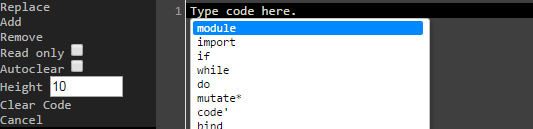
\includegraphics[width=0.9\textwidth]{editor-menu}
\caption{Visual editor's context menu}
\label{fig:editor-menu}
\end{figure}

\section{Visual editor and representation}
The visual representation is implemented in a in terms of a \acrshort{dom} tree, which mirrors the EST: every EST node has a corresponding set of \acrshort{dom} nodes. Thanks to this, any actions performed on the DOM can be tracked through the standard browser-implemented interface. This is done by
attaching \texttt{click} event handlers to relevant nodes. Such an event
triggers the following:
\begin{itemize}
    \item A corresponding EST node is ``focused'' by the system.
    \item The visual node is highlighted.
    \item A context menu appears similar to that depicted in
      \ref{fig:editor-menu}.
\end{itemize}

The context menu depicted in Figure \ref{fig:editor-menu} has all the basic options for manipulating the visual representation. These perform their corresponding action on the currently focused node and propagate it to the text representation. The options are named Replace, Add, and Remove.

The Remove option simply removes the selected node and its subtree from the
DOM, the EST, as well as the associated text fragment.

The Add and Replace options make use of the small text-editor area next to the context menu. It contains a predefined list of names of some of the possible nodes that can be inserted. Selecting any of the names causes a template for the new node -- in the form of an editable code snippet -- to be inserted into the text-editor area. Such a template can be quickly adjusted by the user before inserting.

The predefined list of names is a stub implementation of the context menu feature described in Section \ref{sec:vis_design}

The user may also type in raw code into the text box, without selecting any templates. After entering the code and selecting the appropriate option, the text is parsed, transformed into TextMarker, EST, and DOM representations. Then all the versions of the fragment are inserted in appropriate places.

The list of possible nodes displayed along with the context menu is implemented
in terms of a simple auto-complete functionality on top of CodeMirror. Every item in the auto-complete list is associated with a fragment of code, which is
basically a signature of the corresponding function. User-defined functions
could be easily automatically added to this list by extracting their signatures
from definitions.

The visual representation is composed purely out of HTML and CSS, which makes its appearance fully customizable.